\scanpage{69}
% archive foliation: 68
\diagram{\begin{tabular}{cl}
U N I V E R S I T E & Montpellier, le 26 Juin 1978\\
DES SCIENCES ET TECHNIQUES &\\
DU LANGUEDOC &\\
\texttt{------------}&\\
Service de la Scolarité &\\
MR/GJ &\\
Diffusion : Liste A &\\
N°:4000 &
\end{tabular}}
\uline{AVIS DE SOUTENANCE D'UNE THESE DE DOCTORAT D'UNIVERSITE}

\uline{Nom et prénom du candidat} : PAYEN Jean-Luc

\uline{Titre de la thèse} : Contribution à l'étude de la protection des surfaces métalliques par les composés oxyfluorés du phosphore V.

\uline{Date, heure et lieu de soutenance prévus} :

13 JUILLET 1978 à 11 Heures\\
Ecole Nationale Supérieure de Chimie.

\uline{Nom du Directeur de thèse} :

Monsieur le Professeur L. COT.

\uline{Désignation du laboratoire où la thèse est préparée} :\\
Laboratoire de Chimie minérale appliquée - Chimie des Matériaux, E. N. S. C. M.

\uline{Analyse de l'ouvrage} :

Les sels de l'anion $\mathrm{PO3F}^{2-}$ peuvent être utilisés lors de l'opé-\\
ration de post-traitement après phosphatation en substitution des sels de chrome VI hautement toxiques.

Une étude de la nature de la surface crée par phosphatation et passivation par K2PO3F a été entreprise par différentes techniques : ESCA,Microscopies électronique , et ionique. Elle montre une réorganisation physico chimique de la couche.

\uline{Durée approximative des recherches ayant abouti à la thèse} : 2 ans

\uline{Composition du jury proposé} :
\diagram{\begin{tabular}{lll}
MM. & : &\\
&M.&MAURIN\\
&L.&COT\\
&P.&DESRE\\
&J.&DURAND\\
&X.&GRANDIN DE L'EPREVIER\\
&B.&PARANT\\
&P.R&PHILIP
\end{tabular}}
Le Secrétaire Général,

\figure{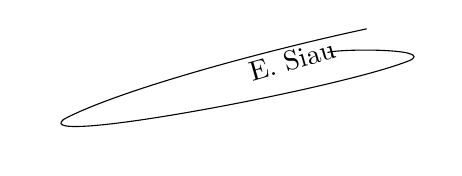
\begin{tikzpicture}[x=1cm,y=1cm]
\node[rotate=16] at (1.55,.3){\unsure{E. Siau}};
\draw (2.5,.7) .. controls (1.1,.4) and (-.7,-.1) .. (-1.35,-.45)
.. controls (-1.8,-.8) and (2.2,-.05) .. (3.05,.3)
.. controls (3.35,.45) and (2.2,.45) .. (2,.4);
\end{tikzpicture}}

\uline{E. SIAU}
